\documentclass[12pt]{article}
\usepackage{graphicx} % Required for inserting images
\usepackage{fullpage}
\usepackage[colorlinks=true,citecolor=blue]{hyperref}
\usepackage{url}
\usepackage{amsmath, amssymb}
\usepackage{amsfonts}
\usepackage{amsthm}
\usepackage{tikz}
\usepackage{CJKutf8}
\usepackage{graphicx} % for \resizebox
\usetikzlibrary{shapes.geometric, arrows.meta}

\usepackage{listings}
\lstset{
  breaklines=true,       % <-- this enables line wrapping
  breakatwhitespace=true,
  basicstyle=\ttfamily,
  frame=single
}

\newtheorem{problem}{Problem}

\title{Gemini 2.5 Pro Capable of Winning Gold at IMO 2025\footnote{Project webpage: \url{https://github.com/lyang36/IMO25}}}
\author{Yichen Huang (黄溢辰)\thanks{\href{mailto:huangtbcmh@gmail.com}{huangtbcmh@gmail.com}} \and Lin F. Yang (杨林)\thanks{\texttt{linyang@ee.ucla.edu}, Department of Electrical and Computer Engineering, and Department of Computer Science, UCLA}}
\date{\today}



\begin{document}
\begin{CJK}{UTF8}{gbsn}
\maketitle
\end{CJK}
\begin{abstract}
The International Mathematical Olympiad (IMO) poses uniquely challenging problems requiring deep insight, creativity, and formal reasoning. While Large Language Models (LLMs) perform well on mathematical benchmarks like AIME, they struggle with Olympiad-level tasks. We use Google’s Gemini 2.5 Pro on the newly released IMO 2025 problems, avoiding data contamination. Using a self-verification pipeline with careful prompt design, 5 (out of 6) problems are solved correctly (up to a caveat discussed below). This result underscores the importance of developing optimal strategies to harness the full potential of powerful LLMs for complex reasoning tasks.
\end{abstract}

\section{Introduction}
The International Mathematical Olympiad (IMO) is an esteemed annual competition that convenes the world's most talented pre-university mathematicians. Established in Romania in 1959 with just seven participating countries, it has since expanded to include over 100 nations, each represented by a team of up to six contestants~\cite{imo_official}. Held annually, with the sole exception of 1980, the IMO challenges participants with exceptionally difficult problems in fields like algebra, geometry, number theory, and combinatorics. Contestants are given two 4.5-hour sessions over two days to solve three problems per session, each graded out of seven points~\cite{djukic2011imo}.
Unlike typical mathematical exercises, IMO problems demand profound insight, originality, and the ability to synthesize diverse mathematical concepts. This emphasis on creative, proof-based reasoning makes the IMO a hallmark of mathematical excellence and a vital platform for identifying future leaders in the field. 

Consequently, the IMO has also become a grand challenge and a formidable benchmark for evaluating the advanced reasoning capabilities of Artificial Intelligence, particularly Large Language Models (LLMs), providing a rigorous test of their ability to perform complex, multi-step logical deduction rather than rote calculation~\cite{han2024olympiadbench, trinh2024alphageometry, matharena2025}. Traditional benchmarks like GSM8K and MATH focus on grade-school and high-school level problems, respectively, where LLMs have achieved high performance through pattern recognition and retrieval from training data~\cite{cobbe2021gsm8k,hendrycks2021math}. However, IMO problems surpass these in complexity, requiring multi-step reasoning, abstraction, and innovation akin to human expert-level cognition, thereby exposing limitations in LLMs’ generalization and vulnerability to hallucinations or superficial heuristics~\cite{frontiermath2024}. This positions the IMO as an ideal probe for assessing whether LLMs can truly ``reason’’ rather than merely replicate memorized solutions, addressing concerns about their reliability in high-stakes domains like scientific discovery and formal verification~\cite{li2025advocate}.

The pursuit of automated mathematical reasoning has seen remarkable progress with the advent of LLMs~\cite{ahn2024large, wang2025survey}. Early successes on foundational benchmarks have rapidly escalated to tackling complex, competition-level mathematics~\cite{liao2023mathagent}. This progress has been significantly propelled by innovations such as Chain-of-Thought (CoT) prompting, which enables models to generate intermediate reasoning steps, thereby improving performance on tasks requiring complex logic and calculation~\cite{wei2022chain}. Nevertheless, even state-of-the-art models have demonstrated significant limitations when confronted with Olympiad-level problems. For example, recent evaluations on problems from the USA Mathematical Olympiad (USAMO) 2025 and IMO 2025 showed that top-tier public models still struggle to produce sound, rigorous proofs and fail to achieve scores comparable to human medalists, often succumbing to logical fallacies and a lack of creative insight~\cite{petrov2025proof, matharena2025}. This highlights a critical gap between generating numerically correct answers and constructing logically sound arguments~\cite{mahdavi2025brains}.

In this paper, we construct a self-verification pipeline with careful prompt design and implemented using the Gemini 2.5 Pro model, a strong base model released by Google~\cite{gemini2025blog}. We solved 5\footnote{Noted that for Problems 1 and 2 we explicitly prompted the model to use induction and analytic geometry. However, these are very general methods. If we had a multi-agent system, we would definitely assign an agent to explore these methods. Thus, it should be clear that Gemini 2.5 Pro has the reasoning capability to win the Gold Medal---hence the title of this paper.} out of the 6 problems of IMO 2025. A persistent and critical challenge in the evaluation of LLMs is the issue of data contamination, where test data from public benchmarks is inadvertently included in the vast pre-training corpora, leading to inflated and unreliable performance metrics~\cite{dodge2021documenting, zhou2024dont}. To ensure a rigorous and uncontaminated assessment of the model’s genuine problem-solving capabilities, this work exclusively utilizes the problems from the most recent IMO 2025 competition. As these problems were released only days before our evaluation, they serve as a pristine testbed, mitigating the risk of data leakage and providing a robust measure of the model’s ability to generalize and reason on genuinely unseen challenges. Our approach shows that strong existing models are already capable of solving difficult math reasoning problems, but directly using them can result in poor results as shown in~\cite{matharena2025}. Our results demonstrate a significant advance in automated mathematical reasoning.

Recently we became aware of an announcement by OpenAI on achieving Gold Medal on IMO 2025~\cite{wei2025openai}. After we submitted this paper to arXiv, we became aware of a similar announcement by Google DeepMind \cite{Deepmind}.

\section{Methods}

\subsection{Pipeline}

At a high level, our pipeline proceeds as follows (illustrated in \ref{fig:flow-diagram}):

\begin{itemize}
    \item Step 1: Initial solution generation with the prompt in Section~\ref{prompt:step1};
    \item Step 2: Self-improvement;
    \item Step 3: Verifying the solution with the prompt in Section~\ref{prompt:verification} and generating a bug report; go to Step 4 or Step 6 (see below for explanations);
    \item Step 4: Review of the bug report;
    \item Step 5: Correcting or improving the solution based on the bug report; go to Step 3;
    \item Step 6: Accept or Reject.
\end{itemize}


\begin{figure}[ht]
\centering
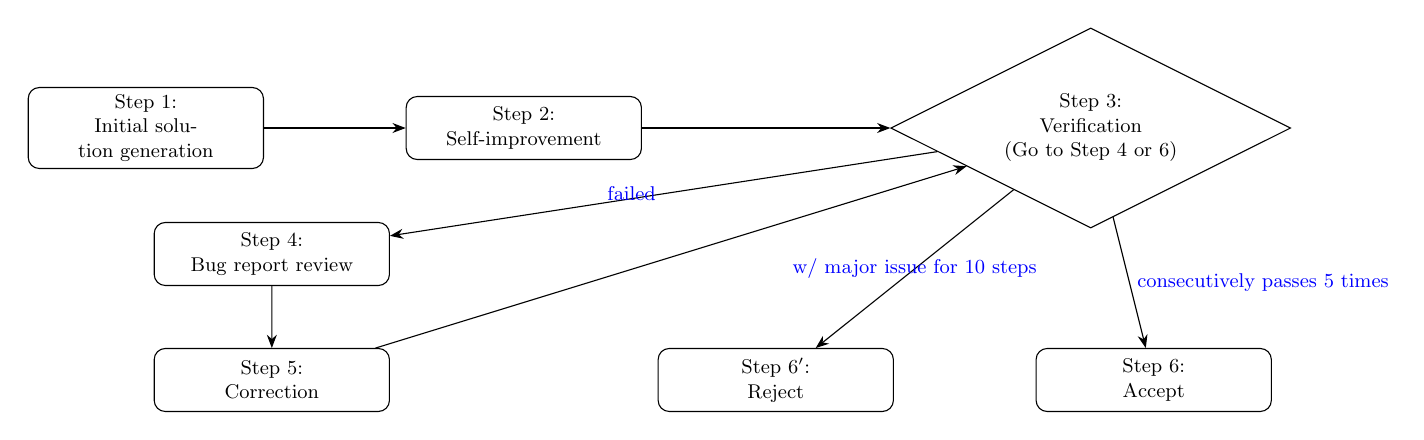
\begin{tikzpicture}[
  scale=0.8,
  transform shape,
  every node/.style={font=\small, align=center},
  process/.style={rectangle, draw, rounded corners, minimum width=3.5cm, minimum height=1cm, text width=3.5cm},
  decision/.style={diamond, draw, aspect=2, inner sep=1pt, minimum height=1.5cm, text width=4cm},
  ->, >=Stealth
  ]

% Nodes (adjusted spacing)
\node[process] (step1) at (0,0) {Step 1:\\ Initial solution generation};
\node[process] (step2) at (6,0) {Step 2:\\ Self-improvement};
\node[decision] (step3) at (15, 0) {Step 3:\\ Verification\\ (Go to Step 4 or 6)};
\node[process] (step4) at (2, -2) {Step 4:\\ Bug report review};
\node[process] (step5) at (2, -4) {Step 5:\\ Correction};
\node[process] (step6) at (16, -4) {Step 6:\\ Accept};
\node[process] (step7) at (10,-4) {Step 6$'$:\\ Reject};

% Arrows
\draw[->] (step1) -- (step2);
\draw[->] (step2) -- (step3);
\draw[->] (step3) -- (step4) node[midway, left] {\textcolor{blue}{failed}};
\draw[->] (step3) -- (step6) node[midway, right] {\textcolor{blue}{consecutively passes 5 times}};
\draw[->] (step3) -- (step7) node[midway] {\textcolor{blue}{w/ major issue for 10 steps}};
\draw[->] (step4) -- (step5);
\draw[->] (step5) -- (step3);

\end{tikzpicture}
\caption{Flow diagram of our pipeline. See the main text for detailed explanations of each step.}
\label{fig:flow-diagram}
\end{figure}

Initially, we run the model (Gemini 2.5 Pro) some number of times and obtain some initial solution samples to the problem. The sampling step is analogous to exploration. We hope that at least one or more samples have some overlap with the correct approach. Then, we try to iteratively improve the solutions and eventually accept high-quality ones.

More specifically, we first have the model attempt to solve the problem with the prompt in Section~\ref{prompt:step1}. This prompt is designed to emphasize rigor rather than focus on finding the final answer and thus matches the theme of IMO. We have randomly selected some outputs and found that the overall quality of the solutions are pretty low. This is consistent with very recent findings of Ref.~\cite{matharena2025}.

In Step 2, the model is prompted to review and try to improve its work. While Gemini 2.5 Pro is good at mathematics, as a general-purpose LLM, it is not tailored to solving especially challenging mathematical problems. One significant constraint is the thinking budget. Note that thinking is quite token consuming: Even a trivial fact might take a few thousand tokens for the model to prove. The maximum number of thinking tokens of Gemini 2.5 Pro is 32768, which is not enough for solving a typical IMO problem. We observe that in Step 1, the model almost always uses up its thinking budget. Thus, the model does not even have the capacity to fully solve the problem. This is why we choose to break down the problem solving process into steps. Step 2 effectively injects another budget of 32768 thinking tokens to allow the model review and continue its work. We keep monitoring the entire process and do observe that the outputs have been noticeably improved during Step 2.

Next we will use the verifier to make iterative improvement and decide whether to accept an improved solution.

\subsection{Verifier}

The verifier plays an important role in our pipeline. Its functionality is to carefully review a solution step by step and find out issues (if any). We emphasize mathematical rigor and classify issues into critical errors and justification gaps. Critical errors are something that is demonstratively false or with clear logical fallacies, while justification gaps can be major or minor. A major justification gap that cannot be repaired would crash an entire proof, while minor justification gaps may not even be well defined: A minor gap could sometimes be viewed as concise argument.

In Step 3, we use the verifier to generate a bug report for each solution outputted in Step 2. The bug report contains a list of issues classified as critical errors or justification gaps. For each issue, an explanation is required. The bug report will serve as useful information for the model to improve the solution, either fixing errors or filling gaps. Step 4 is to carefully review each issue in the bug report. If the verifier makes a mistake and reports an issue which is not really an issue, the issue would be deleted from the bug report. Thus, Step 4 increases the reliability of the bug report. In Step 5, the model tries to improve the solution based on the bug report. We iterate Steps 3-5 a sufficient number of times until we decide to accept or decline a solution. We accept a solution if it robustly passes the verification process and decline a solution if there are always critical errors or major justification gaps during the iterations.

We observe that the verifier is quite reliable but can make mistakes. Since our major goal is not to benchmark the verifier, we do not have quantitative results on its effectiveness. However, we have used this verifier for quite a while (starting from well before IMO 2025). We have been keeping an eye on its performance and below is our qualitative observation:
\begin{itemize}
    \item Critical errors are seldom missed by the verifier. This is consistent with the observations in Ref.~\cite{SLJ15}. In the unlikely event such errors are not caught, simply running the verifier a few more times would very likely catch it. This is good because we do not wish to miss critical errors.
    \item If the verifier reports a critical error, it may not always be critical, but it almost always needs some revision.
    \item The verifier may report some justification gaps which are only slightly beyond trivial statements and thus are not really gaps for mathematicians.
\end{itemize}
Indeed, our system is quite robust to errors made by the verifier. We iteratively use the verifier a sufficiently number of times. If it misses an error in one iteration, it still has some probability to catch it in the next iteration. Also, if it claims an error which is actually not an error, such a false negative may not go through the bug report review step (Step 4). Furthermore, we instruct the model (who generates the solution) to review each item in the bug report. If the model does not agree with a particular item, it is encouraged to revise its solution to minimize misunderstanding. This is analogues to the peer review process. If a referee makes a wrong judgment, the authors are encouraged to revise the paper. Ultimately, the presentation is improved.

At the time we plan to accept a solution, we do not wish the verifier misses any issue; we run the verifier five times and accept a solution only if it passes every time.

\section{Experiment Setup}
We choose low temperature: $0.1$. High temperature may lead to more random errors, which may be harmful. We use the maximum thinking budget ($32768$ reasoning tokens) of Gemini 2.5 Pro. We do not use web search (of course), code, or any other tools. We share the most important prompts below.

\subsection{Step 1 Prompt}
\label{prompt:step1}
\begin{lstlisting}
    ### Core Instructions ###

*   **Rigor is Paramount:** Your primary goal is to produce a complete and rigorously justified solution. Every step in your solution must be logically sound and clearly explained. A correct final answer derived from flawed or incomplete reasoning is considered a failure.
*   **Honesty About Completeness:** If you cannot find a complete solution, you must **not** guess or create a solution that appears correct but contains hidden flaws or justification gaps. Instead, you should present only significant partial results that you can rigorously prove. A partial result is considered significant if it represents a substantial advancement toward a full solution. Examples include:
    *   Proving a key lemma.
    *   Fully resolving one or more cases within a logically sound case-based proof.
    *   Establishing a critical property of the mathematical objects in the problem.
    *   For an optimization problem, proving an upper or lower bound without proving that this bound is achievable.
*   **Use TeX for All Mathematics:** All mathematical variables, expressions, and relations must be enclosed in TeX delimiters (e.g., `Let $n$ be an integer.`).

### Output Format ###

Your response MUST be structured into the following sections, in this exact order.

**1. Summary**

Provide a concise overview of your findings. This section must contain two parts:

*   **a. Verdict:** State clearly whether you have found a complete solution or a partial solution.
    *   **For a complete solution:** State the final answer, e.g., "I have successfully solved the problem. The final answer is..."
    *   **For a partial solution:** State the main rigorous conclusion(s) you were able to prove, e.g., "I have not found a complete solution, but I have rigorously proven that..."
*   **b. Method Sketch:** Present a high-level, conceptual outline of your solution. This sketch should allow an expert to understand the logical flow of your argument without reading the full detail. It should include:
    *   A narrative of your overall strategy.
    *   The full and precise mathematical statements of any key lemmas or major intermediate results.
    *   If applicable, describe any key constructions or case splits that form the backbone of your argument.

**2. Detailed Solution**

Present the full, step-by-step mathematical proof. Each step must be logically justified and clearly explained. The level of detail should be sufficient for an expert to verify the correctness of your reasoning without needing to fill in any gaps. This section must contain ONLY the complete, rigorous proof, free of any internal commentary, alternative approaches, or failed attempts.

### Self-Correction Instruction ###

Before finalizing your output, carefully review your "Method Sketch" and "Detailed Solution" to ensure they are clean, rigorous, and strictly adhere to all instructions provided above. Verify that every statement contributes directly to the final, coherent mathematical argument.
\end{lstlisting}

\subsection{Verification Prompt}
\label{prompt:verification}
\begin{lstlisting}
    You are an expert mathematician and a meticulous grader for an International Mathematical Olympiad (IMO) level exam. Your primary task is to rigorously verify the provided mathematical solution. A solution is to be judged correct **only if every step is rigorously justified.** A solution that arrives at a correct final answer through flawed reasoning, educated guesses, or with gaps in its arguments must be flagged as incorrect or incomplete.

### Instructions ###

**1. Core Instructions**
*   Your sole task is to find and report all issues in the provided solution. You must act as a **verifier**, NOT a solver. **Do NOT attempt to correct the errors or fill the gaps you find.**
*   You must perform a **step-by-step** check of the entire solution. This analysis will be presented in a **Detailed Verification Log**, where you justify your assessment of each step: for correct steps, a brief justification suffices; for steps with errors or gaps, you must provide a detailed explanation.

**2. How to Handle Issues in the Solution**
When you identify an issue in a step, you MUST first classify it into one of the following two categories and then follow the specified procedure.

*   **a. Critical Error:**
    This is any error that breaks the logical chain of the proof. This includes both **logical fallacies** (e.g., claiming that `A>B, C>D` implies `A-C>B-D`) and **factual errors** (e.g., a calculation error like `2+3=6`).
    *   **Procedure:**
        *   Explain the specific error and state that it **invalidates the current line of reasoning**.
        *   Do NOT check any further steps that rely on this error.
        *   You MUST, however, scan the rest of the solution to identify and verify any fully independent parts. For example, if a proof is split into multiple cases, an error in one case does not prevent you from checking the other cases.

*   **b. Justification Gap:**
    This is for steps where the conclusion may be correct, but the provided argument is incomplete, hand-wavy, or lacks sufficient rigor.
    *   **Procedure:**
        *   Explain the gap in the justification.
        *   State that you will **assume the step's conclusion is true** for the sake of argument.
        *   Then, proceed to verify all subsequent steps to check if the remainder of the argument is sound.

**3. Output Format**
Your response MUST be structured into two main sections: a **Summary** followed by the **Detailed Verification Log**.

*   **a. Summary**
    This section MUST be at the very beginning of your response. It must contain two components:
    *   **Final Verdict**: A single, clear sentence declaring the overall validity of the solution. For example: "The solution is correct," "The solution contains a Critical Error and is therefore invalid," or "The solution's approach is viable but contains several Justification Gaps."
    *   **List of Findings**: A bulleted list that summarizes **every** issue you discovered. For each finding, you must provide:
        *   **Location:** A direct quote of the key phrase or equation where the issue occurs.
        *   **Issue:** A brief description of the problem and its classification (**Critical Error** or **Justification Gap**).

*   **b. Detailed Verification Log**
    Following the summary, provide the full, step-by-step verification log as defined in the Core Instructions. When you refer to a specific part of the solution, **quote the relevant text** to make your reference clear before providing your detailed analysis of that part.

**Example of the Required Summary Format**
*This is a generic example to illustrate the required format. Your findings must be based on the actual solution provided below.*

**Final Verdict:** The solution is **invalid** because it contains a Critical Error.

**List of Findings:**
*   **Location:** "By interchanging the limit and the integral, we get..."
    *   **Issue:** Justification Gap - The solution interchanges a limit and an integral without providing justification, such as proving uniform convergence.
*   **Location:** "From $A > B$ and $C > D$, it follows that $A-C > B-D$"
    *   **Issue:** Critical Error - This step is a logical fallacy. Subtracting inequalities in this manner is not a valid mathematical operation.

======================================================================
### Problem ###

[Paste the TeX for the problem statement here]

======================================================================
### Solution ###

[Paste the TeX for the solution to be verified here]

======================================================================
### Verification Task Reminder ###

Your task is to act as an IMO grader. Now, generate the **summary** and the **step-by-step verification log** for the solution above. In your log, justify each correct step and explain in detail any errors or justification gaps you find, as specified in the instructions above.
\end{lstlisting}

\section{Discussions on IMO 2025 Problems}

\begin{problem}
A line in the plane is called \textit{sunny} if it is not parallel to any of the $x$-axis, the $y$-axis, and the line $x+y=0$.

Let $n \ge 3$ be a given integer. Determine all nonnegative integers $k$ such that there exist $n$ distinct lines in the plane satisfying both the following:
\begin{itemize}
    \item For all positive integers $a$ and $b$ with $a + b \le n + 1$, the point $(a,b)$ is on at least one of the lines; and
    \item Exactly $k$ of the lines are sunny.
\end{itemize}
\end{problem}

Immediately after sending the problem statement to the model, we added an extra sentence ``\emph{Let us try to solve the problem by induction.}'' Does this sentence provide hint or guidance to the model? The answer is both yes and no. This combinatorial problem can be solved by mathematical induction. Thus, the extra sentence is certainly helpful in the sense of pointing the model to the correct direction.

However, one can also argue that the italicized sentence (as a prompt) does not provide any essential help other than reducing computational resource usage. Imagine you have a multi-agent system aiming at solving a difficult problem. Such task usually requires a lot of exploration: One should have different agents try different methods in the hope that one of them can find a promising path. For any proposition that holds for positive integers, mathematical induction is a standard and often effective method. Thus, a multi-agent system should assign at least one agent to consider induction if it looks like a viable approach. After all, induction is very general technique, not limited to the problem we are trying to solve.

\begin{problem}
Let $\Omega$ and $\Gamma$ be circles with centers $M$ and $N$, respectively, such that the radius of $\Omega$ is less than the radius of $\Gamma$. Suppose circles $\Omega$ and $\Gamma$ intersect at two distinct points $A$ and $B$. Let $MN$ intersect $\Omega$ at $C$ and $\Gamma$ at $D$, such that points $C$, $M$, $N$, and $D$ lie on the line in that order. Let $P$ be the circumcenter of triangle $ACD$. Line $AP$ intersects $\Omega$ again at $E \ne A$. Line $AP$ intersects $\Gamma$ again at $F \ne A$. Let $H$ be the orthocenter of triangle $PMN$.

Prove that the line through $H$ parallel to $AP$ is tangent to the circumcircle of triangle $BEF$.

(The orthocenter of a triangle is the point of intersection of its altitudes.)
\end{problem}

Immediately after sending the problem statement to the model, we added an extra sentence ``\emph{Let us try to solve the problem by analytic geometry.}'' Discussions similar to those under the preceding problem apply here. We acknowledge that this sentence provides hint to the model, but still argue that its major effect is to reduce computational resource usage. Analytic geometry is a quite general method for solving high-school geometry problems as long as the calculations are not too complicated. It is an idea that deserves a try.

Large language models are actually good at doing straightforward calculations. For this particular problem, on our first try Gemini 2.5 Pro already gave us an almost correct answer up to some small calculation mistakes that were subsequently caught by the verifier. For AI, this is the easiest problem in IMO 2025.

\begin{problem}
Let $\mathbb{N}$ denote the set of positive integers. A function $f : \mathbb{N} \to \mathbb{N}$ is said to be \textit{bonza} if
\[
f(a) \mid b^a - f(b)^{f(a)}
\]
for all positive integers $a$ and $b$.

Determine the smallest real constant $c$ such that $f(n) \le cn$ for all bonza functions $f$ and all positive integers $n$.
\end{problem}

Our pipeline is to sample a sufficient number of initial solutions and then make improvements iteratively. For this problem, we sampled $20$ times and succeeded in obtaining a rigorous solution within our approach. Note that MathAerna \cite{matharena2025} observed that if sampling $32$ times, one can directly get a rigorous solution with $50\%$ probability. We do not need to sample this many times because we iteratively improve our solution. For us, as long as the initial solution has substantial overlap with a correct approach, there is hope that we can succeed.

We do not have specific comments for the three problems below. We include the problem statements for completeness.

\begin{problem}
A proper divisor of a positive integer $N$ is a positive divisor of $N$ other than $N$ itself.

The infinite sequence $a_1, a_2, \ldots$ consists of positive integers, each of which has at least three proper divisors. For each $n \ge 1$, the integer $a_{n+1}$ is the sum of the three largest proper divisors of $a_n$.

Determine all possible values of $a_1$.
\end{problem}

\begin{problem}
Alice and Bazza are playing the \textit{inekoalaty} game, a two-player game whose rules depend on a positive real number $\lambda$ which is known to both players. On the $n$th turn of the game (starting with $n = 1$) the following happens:
\begin{itemize}
    \item If $n$ is odd, Alice chooses a nonnegative real number $x_n$ such that
    \[
    x_1 + x_2 + \cdots + x_n \le \lambda n.
    \]
    \item If $n$ is even, Bazza chooses a nonnegative real number $x_n$ such that 
    \[
    x_1^2 + x_2^2 + \cdots + x_n^2 \le n.
    \]
\end{itemize}

If a player cannot choose a suitable number $x_n$, the game ends and the other player wins. If the game goes forever, neither player wins. All chosen numbers are known to both players.

Determine all values of $\lambda$ for which Alice has a winning strategy and all those for which Bazza has a winning strategy.
\end{problem}

\begin{problem}
Consider a $2025 \times 2025$ grid of unit squares. Matilda wishes to place on the grid some rectangular tiles, possibly of different sizes, such that each side of every tile lies on a grid line and every unit square is covered by at most one tile.

Determine the minimum number of tiles Matilda needs to place so that each row and each column of the grid has exactly one unit square that is not covered by any tile.
\end{problem}

\section{Gemini 2.5 Pro Solutions to the Problems}

The solutions outputted by Gemini 2.5 Pro are in a combination of Markdown and TeX format. Problems 1-5 are solved.

\subsection{Problem 1}

Let $S_n = \{(a,b) \in \mathbb{Z}^2 \mid a \ge 1, b \ge 1, a+b \le n+1\}$. A line is *sunny* if its slope is not $0, \infty,$ or $-1$. We seek the set of non-negative integers $k$ such that for a given integer $n \ge 3$, there exist $n$ distinct lines covering $S_n$, exactly $k$ of which are sunny.

**Part 1: Reduction to a Core Problem**

Let $\mathcal{L}$ be a set of $n$ distinct lines covering $S_n$. The *principal boundary lines* of $S_n$ are the lines $x=1$, $y=1$, and $x+y=n+1$. These are all non-sunny.

**Lemma:** If a principal boundary line $L$ of $S_n$ is in $\mathcal{L}$, then there exists a set of $n-1$ distinct lines $\mathcal{L}'$ that covers $S_{n-1}$ and has the same number of sunny lines as $\mathcal{L}$.

*Proof.* Let $k$ be the number of sunny lines in $\mathcal{L}$. The line $L$ is not sunny.
1.  Suppose $L$ is the line $x=1$. This line covers the points $\{(1,b) \mid 1 \le b \le n\}$. The remaining $n-1$ lines in $\mathcal{L} \setminus \{L\}$ must cover the set $S'_n = \{(a,b) \in S_n \mid a \ge 2\}$. The affine transformation $\phi(a,b) = (a-1, b)$ is a bijection from $S'_n$ to $S_{n-1}$. Let $\mathcal{L}'$ be the set of lines obtained by transforming the lines in $\mathcal{L} \setminus \{L\}$. A point $(x',y')$ is on a transformed line $l'$ if its pre-image under $\phi$, which is $(x'+1, y')$, is on the original line $l$. If $l$ has equation $Ax+By+C=0$, the transformed line $l'$ has equation $A(x+1)+By+C=0$. This transformation preserves the slope of any line, so the number of sunny lines in $\mathcal{L}'$ is $k$. The lines in $\mathcal{L}'$ are distinct: if $l_1: A_1x+B_1y+C_1=0$ and $l_2: A_2x+B_2y+C_2=0$ are distinct lines in $\mathcal{L} \setminus \{L\}$, their images are $l'_1: A_1x+B_1y+(A_1+C_1)=0$ and $l'_2: A_2x+B_2y+(A_2+C_2)=0$. If $l'_1=l'_2$, their coefficients are proportional, so $(A_1, B_1, A_1+C_1) = \lambda(A_2, B_2, A_2+C_2)$ for some $\lambda \ne 0$. This implies $A_1=\lambda A_2$, $B_1=\lambda B_2$, and $A_1+C_1=\lambda(A_2+C_2)$. Substituting the first into the third gives $\lambda A_2+C_1=\lambda A_2+\lambda C_2$, so $C_1=\lambda C_2$. Thus $(A_1,B_1,C_1)=\lambda(A_2,B_2,C_2)$, contradicting the distinctness of $l_1, l_2$.
2.  If $L$ is $y=1$, a symmetric argument with the transformation $(a,b) \mapsto (a, b-1)$ applies.
3.  If $L$ is $x+y=n+1$, it covers the points $\{(a,b) \in S_n \mid a+b=n+1\}$. The other $n-1$ lines must cover the remaining points, which form the set $\{(a,b) \in S_n \mid a+b \le n\} = S_{n-1}$. Thus, $\mathcal{L}' = \mathcal{L} \setminus \{L\}$ is a set of $n-1$ distinct lines covering $S_{n-1}$ with $k$ sunny lines.

By repeatedly applying this lemma, any configuration for $S_n$ can be reduced. This process terminates when we obtain a set of $m$ lines covering $S_m$ (for some $m \le n$) where none of the lines are principal boundary lines of $S_m$. The number of sunny lines in this new configuration is still $k$.

Let $\mathcal{L}_m$ be such a set of $m$ lines covering $S_m$.
Let $C_{m,x} = \{(1,b) \mid 1 \le b \le m\}$. These $m$ points must be covered by $\mathcal{L}_m$. Since $x=1 \notin \mathcal{L}_m$, any vertical line in $\mathcal{L}_m$ (of the form $x=c, c \ne 1$) misses all points in $C_{m,x}$. Each of the non-vertical lines in $\mathcal{L}_m$ can cover at most one point of $C_{m,x}$. If there are $v$ vertical lines in $\mathcal{L}_m$, then the remaining $m-v$ lines must cover all $m$ points, so $m-v \ge m$, which implies $v=0$. Thus, $\mathcal{L}_m$ contains no vertical lines (slope $\infty$).
By a symmetric argument considering $C_{m,y} = \{(a,1) \mid 1 \le a \le m\}$, we deduce $\mathcal{L}_m$ contains no horizontal lines (slope $0$).
By considering $C_{m,sum} = \{(a,b) \in S_m \mid a+b=m+1\}$, we deduce $\mathcal{L}_m$ contains no lines of slope $-1$.
Therefore, all $m$ lines in $\mathcal{L}_m$ must be sunny. This implies $k=m$. The problem reduces to finding for which non-negative integers $k$ it is possible to cover $S_k$ with $k$ distinct sunny lines, none of which are principal boundary lines of $S_k$.

**Part 2: Analysis of the Core Problem**

*   **$k=0$:** $S_0 = \emptyset$. This is covered by 0 lines. So $k=0$ is possible.
*   **$k=1$:** $S_1 = \{(1,1)\}$. The line $y=x$ is sunny, covers $(1,1)$, and is not a principal boundary line of $S_1$ (which are $x=1, y=1, x+y=2$). So $k=1$ is possible.
*   **$k=2$:** $S_2 = \{(1,1), (1,2), (2,1)\}$. We need to cover these three points with two distinct sunny lines, neither of which can be a principal boundary line of $S_2$ ($x=1, y=1, x+y=3$). A line passing through any two of the points in $S_2$ must be one of these three principal boundary lines, which are non-sunny. Therefore, a sunny line can pass through at most one point of $S_2$. Consequently, two sunny lines can cover at most two points, leaving at least one point of $S_2$ uncovered. So $k=2$ is impossible.
*   **$k=3$:** $S_3 = \{(1,1), (1,2), (1,3), (2,1), (2,2), (3,1)\}$. The following three lines are sunny, distinct, not principal boundary lines of $S_3$, and cover $S_3$:
    $L_1: y = -2x+5$ (covers $(1,3), (2,1)$)
    $L_2: y = x$ (covers $(1,1), (2,2)$)
    $L_3: x+2y=5$ (covers $(1,2), (3,1)$)
    So $k=3$ is possible.
*   **$k \ge 4$:** Assume there exists a set $\mathcal{L}$ of $k$ distinct sunny lines covering $S_k$, with no principal boundary lines. As argued, each line in $\mathcal{L}$ must intersect each of the sets $C_y=\{(i,1)\}_{i=1}^k$, $C_x=\{(1,j)\}_{j=1}^k$, and $C_s=\{(p,k+1-p)\}_{p=1}^k$ at exactly one point.
    We can label the lines $L_i$ for $i \in \{1, \dots, k\}$ such that $L_i$ is the unique line in $\mathcal{L}$ passing through $(i,1)$. For each $i$, $L_i$ must also pass through a unique point $(1, \sigma(i)) \in C_x$ and a unique point $(\pi(i), k+1-\pi(i)) \in C_s$. The maps $\sigma, \pi: \{1, \dots, k\} \to \{1, \dots, k\}$ must be permutations.

    These permutations must satisfy several properties:
    1.  $L_1$ passes through $(1,1)$, so $\sigma(1)=1$.
    2.  $L_k$ passes through $(k,1)$, which is also in $C_s$. Thus, $(\pi(k), k+1-\pi(k))=(k,1)$, which implies $\pi(k)=k$.
    3.  There is a unique line $L_j$ passing through $(1,k) \in C_x$, so $\sigma(j)=k$. The point $(1,k)$ is also in $C_s$, so for $L_j$, $(\pi(j), k+1-\pi(j))=(1,k)$, which implies $\pi(j)=1$. Since $\sigma(1)=1 \ne k$ and $\pi(k)=k \ne 1$, we have $j \ne 1,k$, so $j \in \{2, \dots, k-1\}$.
    4.  For $i \in \{2, \dots, k\}$, if $\sigma(i)=i$, $L_i$ would pass through $(i,1)$ and $(1,i)$, giving it slope $-1$, which is not allowed. So $\sigma(i) \ne i$ for $i \ge 2$.
    5.  For $i \in \{1, \dots, k-1\}$, if $\pi(i)=i$, $L_i$ would pass through $(i,1)$ and $(i, k+1-i)$, making it a vertical line, which is not allowed. So $\pi(i) \ne i$ for $i \le k-1$.

    For any $i \in \{1, \dots, k\}$, the three points $P_1=(i,1)$, $P_2=(1, \sigma(i))$, and $P_3=(\pi(i), k+1-\pi(i))$ must be collinear. For $i \in \{2, \dots, k-1\} \setminus \{j\}$, these three points are distinct. To prove this:
    - $P_1=P_2 \implies i=1$, but $i \ge 2$.
    - $P_1=P_3 \implies \pi(i)=i$, but $\pi(i) \ne i$ for $i \le k-1$.
    - $P_2=P_3 \implies \pi(i)=1$ and $\sigma(i)=k$. By definition of $j$, this means $i=j$. But we consider $i \ne j$.
    Thus, for $i \in \{2, \dots, k-1\} \setminus \{j\}$, the points are distinct. Collinearity implies their slopes are equal: $\frac{\sigma(i)-1}{1-i} = \frac{k+1-\pi(i)-1}{\pi(i)-i}$. This gives $\sigma(i) = 1 + (i-1)\frac{k-\pi(i)}{i-\pi(i)}$.

    **Step 1: Show $j=k-1$.**
    Assume for contradiction that $j \ne k-1$. Then the formula for $\sigma(i)$ is valid for $i=k-1$.
    $\sigma(k-1) = 1 + (k-2)\frac{k-\pi(k-1)}{k-1-\pi(k-1)}$.
    From the properties of $\pi$: $\pi(k-1) \in \{1, \dots, k\}$, $\pi(k-1) \ne \pi(j)=1$, $\pi(k-1) \ne \pi(k)=k$, and $\pi(k-1) \ne k-1$. So $\pi(k-1) \in \{2, \dots, k-2\}$.
    Let $d = k-1-\pi(k-1)$. Then $d \in \{1, \dots, k-3\}$.
    $\sigma(k-1) = 1 + (k-2)\frac{k-(k-1-d)}{d} = 1 + (k-2)\frac{d+1}{d} = 1+(k-2)(1+\frac{1}{d}) = k-1 + \frac{k-2}{d}$.
    Since $k \ge 4$, we have $d \le k-3$, so $\frac{k-2}{d} \ge \frac{k-2}{k-3} = 1+\frac{1}{k-3} > 1$.
    So $\sigma(k-1) > k-1+1=k$. This contradicts $\sigma(k-1) \in \{1, \dots, k\}$.
    Thus, our assumption was false. We must have $j=k-1$.

    **Step 2: Derive a final contradiction.**
    We have established that for $k \ge 4$, it must be that $j=k-1$, which means $\sigma(k-1)=k$ and $\pi(k-1)=1$.
    Consider $i=2$. Since $k \ge 4$, $j=k-1 \ge 3$, so $j \ne 2$. The formula for $\sigma(i)$ is valid for $i=2$:
    $\sigma(2) = 1 + \frac{k-\pi(2)}{2-\pi(2)}$.
    Since $\pi$ is a permutation, its image on $\{1, \dots, k-2\}$ is $\{1, \dots, k\} \setminus \{\pi(k-1), \pi(k)\}$. With $\pi(k-1)=1$ and $\pi(k)=k$, we have $\pi(\{1, \dots, k-2\}) = \{2, \dots, k-1\}$.
    So $\pi(2) \in \{2, \dots, k-1\}$. By property 5, $\pi(2) \ne 2$. Thus $\pi(2) \in \{3, \dots, k-1\}$.
    Let $d' = \pi(2)-2$. Then $d' \in \{1, \dots, k-3\}$.
    The denominator is $2-\pi(2) = -d'$.
    $\sigma(2) = 1 + \frac{k-(d'+2)}{-d'} = 1 - \frac{k-d'-2}{d'} = 1 - \left(\frac{k-2}{d'}-1\right) = 2 - \frac{k-2}{d'}$.
    Since $d' \le k-3$, we have $\frac{k-2}{d'} \ge \frac{k-2}{k-3} = 1+\frac{1}{k-3} > 1$ for $k \ge 4$.
    So $\sigma(2) = 2 - \frac{k-2}{d'} < 2-1=1$.
    This contradicts $\sigma(2) \in \{1, \dots, k\}$.
    This final contradiction shows that no such configuration is possible for $k \ge 4$.

**Part 3: Constructions for general $n \ge 3$**

The set of possible values for $k$ is $\{0, 1, 3\}$. We now show these are all possible for any $n \ge 3$.

*   **$k=0$:** Let $\mathcal{L} = \{x=i \mid i=1, 2, \dots, n\}$. These are $n$ distinct non-sunny lines. Any point $(a,b) \in S_n$ has $1 \le a \le n$, so it lies on the line $x=a \in \mathcal{L}$.
*   **$k=1$:** Let $\mathcal{L} = \{x=i \mid i=1, \dots, n-1\} \cup \{y=x-(n-1)\}$. The first $n-1$ lines are non-sunny and cover all points $(a,b) \in S_n$ with $a \le n-1$. The only points in $S_n$ not covered are those with $a \ge n$. If $(a,b) \in S_n$ and $a \ge n$, then $n+b \le a+b \le n+1$, which implies $b \le 1$. Since $b \ge 1$, we must have $b=1$. Then $a+1 \le n+1 \implies a \le n$. The only uncovered point is $(n,1)$. The line $y=x-(n-1)$ has slope 1 (sunny), is distinct from the other lines, and passes through $(n,1)$ since $1 = n-(n-1)$.
*   **$k=3$:** Let $\mathcal{L}_{ns} = \{x+y=c \mid c=5, 6, \dots, n+1\}$. This is a set of $n-3$ distinct non-sunny lines (if $n=3$, this set is empty). These lines cover all points $(a,b) \in S_n$ with $a+b \ge 5$. The remaining points to be covered are $U = \{(a,b) \in S_n \mid a+b \le 4\}$. This set is precisely $S_3$. As shown in Part 2, $S_3$ can be covered by 3 distinct sunny lines. Let $\mathcal{L}_s$ be this set of 3 lines. Then $\mathcal{L} = \mathcal{L}_{ns} \cup \mathcal{L}_s$ is a set of $(n-3)+3=n$ lines covering $S_n$. The lines in $\mathcal{L}_s$ have slopes different from $-1$, so they are distinct from lines in $\mathcal{L}_{ns}$. This construction provides exactly 3 sunny lines.

Thus, for any integer $n \ge 3$, configurations with $k \in \{0, 1, 3\}$ sunny lines are possible.

\subsection{Problem 2}

**1. Coordinate System and Geometric Setup**

We establish a Cartesian coordinate system. Let the line of centers $MN$ be the $x$-axis, and the common chord $AB$ be the $y$-axis. Let their intersection be the origin $O(0,0)$.

*   The points of intersection of the circles are $A(0,a)$ and $B(0,-a)$ for some $a>0$.
*   The centers of the circles are $M(m,0)$ and $N(n,0)$.
*   Circle $\Omega$ has center $M(m,0)$ and passes through $A(0,a)$. Its radius is $R_\Omega = \sqrt{m^2+a^2}$. The equation of $\Omega$ is $(x-m)^2+y^2 = m^2+a^2$, which simplifies to $x^2-2mx+y^2=a^2$.
*   Circle $\Gamma$ has center $N(n,0)$ and passes through $A(0,a)$. Its radius is $R_\Gamma = \sqrt{n^2+a^2}$. The equation of $\Gamma$ is $(x-n)^2+y^2 = n^2+a^2$, which simplifies to $x^2-2nx+y^2=a^2$.
*   The line $MN$ is the $x$-axis. The points $C$ and $D$ lie on the $x$-axis. Let their coordinates be $C(c,0)$ and $D(d,0)$.
*   The condition that $C, M, N, D$ lie on the line in that order implies their $x$-coordinates are ordered: $c < m < n < d$.
*   $C$ is an intersection of $\Omega$ with the $x$-axis. Its coordinate $c$ is a root of $x^2-2mx-a^2=0$. The roots are $m \pm \sqrt{m^2+a^2}$. Since $c<m$, we must have $c = m-\sqrt{m^2+a^2}$.
*   $D$ is an intersection of $\Gamma$ with the $x$-axis. Its coordinate $d$ is a root of $x^2-2nx-a^2=0$. The roots are $n \pm \sqrt{n^2+a^2}$. Since $d>n$, we must have $d=n+\sqrt{n^2+a^2}$.
*   From the equations for $c$ and $d$, we have $c^2-2mc-a^2=0$ and $d^2-2nd-a^2=0$. Since $c<0$ and $d>0$, $c,d \neq 0$. We can express $m$ and $n$ as:
    $m = \frac{c^2-a^2}{2c}$ and $n = \frac{d^2-a^2}{2d}$.

**2. Preliminary Geometric and Algebraic Properties**

We establish two key properties derived from the problem's conditions.

*   **Lemma 1:** $c+d \neq 0$.
    *   **Proof:** The condition $R_\Omega < R_\Gamma$ implies $m^2+a^2 < n^2+a^2$, so $m^2 < n^2$.
    *   The ordering $C,M,N,D$ implies $m<n$.
    *   From $m<n$ and $m^2<n^2$, we have $n^2-m^2 > 0$, so $(n-m)(n+m)>0$. Since $n-m>0$, we must have $n+m>0$.
    *   Also, $m^2 < n^2 \implies m^2+a^2 < n^2+a^2 \implies \sqrt{m^2+a^2} < \sqrt{n^2+a^2}$.
    *   Assume for contradiction that $c+d=0$. Using the expressions for $c$ and $d$:
        $(m-\sqrt{m^2+a^2}) + (n+\sqrt{n^2+a^2}) = 0 \implies m+n = \sqrt{m^2+a^2} - \sqrt{n^2+a^2}$.
    *   The left side, $m+n$, is positive. The right side, $\sqrt{m^2+a^2} - \sqrt{n^2+a^2}$, is negative. This is a contradiction.
    *   Thus, our assumption is false, and $c+d \neq 0$.

*   **Lemma 2:** $a^2+cd < 0$.
    *   **Proof:** The condition $m<n$ implies $\frac{c^2-a^2}{2c} < \frac{d^2-a^2}{2d}$.
    *   From their definitions, $c<0$ and $d>0$, so $cd<0$. Multiplying the inequality by $2cd$ (which is negative) reverses the inequality sign:
        $d(c^2-a^2) > c(d^2-a^2) \implies c^2d-a^2d > cd^2-a^2c \implies cd(c-d) > -a^2(c-d)$.
    *   Since $c<d$, we have $c-d<0$. Dividing by $c-d$ reverses the inequality sign again:
        $cd < -a^2 \implies a^2+cd < 0$.

**3. Coordinates of P and H**

*   Let $P(x_P, y_P)$ be the circumcenter of $\triangle ACD$ with vertices $A(0,a)$, $C(c,0)$, $D(d,0)$.
*   $P$ lies on the perpendicular bisector of segment $CD$, which is the line $x = \frac{c+d}{2}$. So, $x_P = \frac{c+d}{2}$.
*   The condition $PA^2 = PC^2$ gives $(x_P-0)^2 + (y_P-a)^2 = (x_P-c)^2 + (y_P-0)^2$.
    $x_P^2 + y_P^2 - 2ay_P + a^2 = x_P^2 - 2cx_P + c^2 + y_P^2 \implies -2ay_P + a^2 = -2cx_P + c^2$.
    Substituting $x_P = \frac{c+d}{2}$: $-2ay_P + a^2 = -c(c+d) + c^2 = -cd \implies y_P = \frac{a^2+cd}{2a}$.
    So, $P\left(\frac{c+d}{2}, \frac{a^2+cd}{2a}\right)$.

*   Let $H(x_H, y_H)$ be the orthocenter of $\triangle PMN$ with vertices $P(x_P, y_P)$, $M(m,0)$, $N(n,0)$.
*   The altitude from $P$ to $MN$ (on the $x$-axis) is the line $x=x_P$. Thus, $x_H = x_P = \frac{c+d}{2}$.
*   The altitude from $M$ is perpendicular to $PN$. The slope of this altitude is $-\frac{x_P-n}{y_P}$. The line is $y-0 = -\frac{x_P-n}{y_P}(x-m)$.
*   $H$ lies on this line, so $y_H = -\frac{x_P-n}{y_P}(x_H-m) = -\frac{(x_P-m)(x_P-n)}{y_P}$.
*   We express the numerator in terms of $a,c,d$:
    $x_P-m = \frac{c+d}{2} - \frac{c^2-a^2}{2c} = \frac{c(c+d)-(c^2-a^2)}{2c} = \frac{cd+a^2}{2c}$.
    $x_P-n = \frac{c+d}{2} - \frac{d^2-a^2}{2d} = \frac{d(c+d)-(d^2-a^2)}{2d} = \frac{cd+a^2}{2d}$.
*   Substituting these into the expression for $y_H$:
    $y_H = -\frac{1}{y_P} \left(\frac{cd+a^2}{2c}\right) \left(\frac{cd+a^2}{2d}\right) = -\frac{(cd+a^2)^2}{4cd y_P}$.
    Using $y_P = \frac{a^2+cd}{2a}$ and $a^2+cd \neq 0$ (from Lemma 2), we get:
    $y_H = -\frac{(cd+a^2)^2}{4cd} \frac{2a}{a^2+cd} = -\frac{a(a^2+cd)}{2cd}$.
*   So, the coordinates of the orthocenter are $H\left(\frac{c+d}{2}, -\frac{a(a^2+cd)}{2cd}\right)$.

**4. The Line AP and its Intersections**

*   Since $a \neq 0$ and $c+d \neq 0$ (Lemma 1), the slope of line $AP$, denoted $k_{AP}$, is well-defined:
    $k_{AP} = \frac{y_P-a}{x_P-0} = \frac{\frac{a^2+cd}{2a}-a}{\frac{c+d}{2}} = \frac{a^2+cd-2a^2}{a(c+d)} = \frac{cd-a^2}{a(c+d)}$.
*   The line $AP$ has equation $y=k_{AP}x+a$. $E(x_E, y_E)$ and $F(x_F, y_F)$ are the other intersection points of this line with $\Omega$ and $\Gamma$ respectively.
*   To find $E$, substitute $y=k_{AP}x+a$ into the equation of $\Omega$, $x^2-2mx+y^2=a^2$:
    $x^2-2mx+(k_{AP}x+a)^2=a^2 \implies x((1+k_{AP}^2)x - 2m + 2ak_{AP})=0$.
    The roots are $x=0$ (for point $A$) and $x_E = \frac{2(m-ak_{AP})}{1+k_{AP}^2}$.
*   Similarly, for $F$ on $\Gamma$ ($x^2-2nx+y^2=a^2$): $x_F = \frac{2(n-ak_{AP})}{1+k_{AP}^2}$.

**5. Auxiliary Algebraic Identities**

We derive identities that will simplify subsequent calculations.
*   **Identity 1:** $m-ak_{AP} = \frac{c^2-a^2}{2c} - a\left(\frac{cd-a^2}{a(c+d)}\right) = \frac{(c^2-a^2)(c+d) - 2c(cd-a^2)}{2c(c+d)} = \frac{(c^2+a^2)(c-d)}{2c(c+d)}$.
*   **Identity 2:** $n-ak_{AP} = \frac{d^2-a^2}{2d} - \frac{cd-a^2}{c+d} = \frac{(d^2-a^2)(c+d) - 2d(cd-a^2)}{2d(c+d)} = \frac{(d^2+a^2)(d-c)}{2d(c+d)}$.
*   **Identity 3:** $1+k_{AP}^2 = 1+\left(\frac{cd-a^2}{a(c+d)}\right)^2 = \frac{a^2(c+d)^2+(cd-a^2)^2}{a^2(c+d)^2} = \frac{(c^2+a^2)(d^2+a^2)}{a^2(c+d)^2}$.
*   **Identity 4:** $k_{AP}+\frac{2a}{x_E} = \frac{cd-a^2}{a(c+d)} + \frac{a(1+k_{AP}^2)}{m-ak_{AP}} = \frac{cd-a^2}{a(c+d)} + a \frac{(c^2+a^2)(d^2+a^2)}{a^2(c+d)^2} \left/ \frac{(c^2+a^2)(c-d)}{2c(c+d)} \right. = \frac{cd-a^2}{a(c+d)} + \frac{2c(d^2+a^2)}{a(c+d)(c-d)} = \frac{(cd-a^2)(c-d)+2c(d^2+a^2)}{a(c+d)(c-d)} = \frac{cd(c+d)+a^2(c+d)}{a(c+d)(c-d)} = \frac{cd+a^2}{a(c-d)}$.

**6. The Circumcircle of $\triangle BEF$**

Let $K(x_K, y_K)$ be the circumcenter of $\triangle BEF$. $K$ lies on the perpendicular bisectors of $BE$ and $BF$.
The perpendicular bisector of $BE$ is given by $KB^2=KE^2$, which simplifies to $2x_Kx_E+2y_K(y_E+a) = x_E^2+y_E^2-a^2+2a^2 = 2mx_E+2a^2$. Using $y_E=k_{AP}x_E+a$, we get $x_Kx_E+y_K(k_{AP}x_E+2a) = mx_E+a^2$. This is incorrect.
Let's re-derive. $KB^2=KE^2 \implies x_K^2+(y_K+a)^2 = (x_K-x_E)^2+(y_K-y_E)^2$.
$x_K^2+y_K^2+2ay_K+a^2 = x_K^2-2x_Kx_E+x_E^2+y_K^2-2y_Ky_E+y_E^2$.
$2ay_K+a^2 = -2x_Kx_E+x_E^2-2y_Ky_E+y_E^2$.
Since $E$ is on $\Omega$, $x_E^2+y_E^2=2mx_E+a^2$.
$2ay_K+a^2 = -2x_Kx_E+2mx_E+a^2-2y_Ky_E$.
$2ay_K = -2x_Kx_E+2mx_E-2y_Ky_E$.
$ay_K = -x_Kx_E+mx_E-y_Ky_E$.
$ay_K = -x_Kx_E+mx_E-y_K(k_{AP}x_E+a) \implies 2ay_K = -x_Kx_E+mx_E-y_Kk_{AP}x_E$.
$x_E(x_K+y_Kk_{AP}) + 2ay_K = mx_E$. Dividing by $x_E \neq 0$:
(1) $x_K + y_K(k_{AP}+\frac{2a}{x_E}) = m$.
A similar derivation for the perpendicular bisector of $BF$ (using point $F$ on $\Gamma$) yields:
(2) $x_K + y_K(k_{AP}+\frac{2a}{x_F}) = n$.
Subtracting (1) from (2): $y_K(\frac{2a}{x_F}-\frac{2a}{x_E}) = n-m \implies 2ay_K\frac{x_E-x_F}{x_Ex_F} = n-m$.
Using $x_E-x_F = \frac{2(m-n)}{1+k_{AP}^2}$, we get $2ay_K \frac{2(m-n)/(1+k_{AP}^2)}{x_Ex_F} = n-m$. Since $m \neq n$, we find $y_K = -\frac{x_Ex_F(1+k_{AP}^2)}{4a} = -\frac{(m-ak_{AP})(n-ak_{AP})}{a(1+k_{AP}^2)}$.
Using Identities 1, 2, 3:
$y_K = -\frac{1}{a} \left(\frac{(c^2+a^2)(c-d)}{2c(c+d)}\right) \left(\frac{(d^2+a^2)(d-c)}{2d(c+d)}\right) \left/ \frac{(c^2+a^2)(d^2+a^2)}{a^2(c+d)^2} \right. = \frac{a(c-d)^2}{4cd}$.
From (1) and Identity 4: $x_K = m - y_K(k_{AP}+\frac{2a}{x_E}) = m - y_K\frac{cd+a^2}{a(c-d)}$.
$x_K = \frac{c^2-a^2}{2c} - \frac{a(c-d)^2}{4cd} \frac{cd+a^2}{a(c-d)} = \frac{c^2-a^2}{2c} - \frac{(c-d)(cd+a^2)}{4cd} = \frac{2d(c^2-a^2) - (c-d)(cd+a^2)}{4cd} = \frac{cd(c+d)-a^2(c+d)}{4cd} = \frac{(cd-a^2)(c+d)}{4cd}$.
The radius squared of the circumcircle of $\triangle BEF$ is $R_K^2 = KB^2 = x_K^2+(y_K+a)^2$.
$y_K+a = \frac{a(c-d)^2}{4cd}+a = \frac{a(c+d)^2}{4cd}$.
$R_K^2 = \left(\frac{(cd-a^2)(c+d)}{4cd}\right)^2 + \left(\frac{a(c+d)^2}{4cd}\right)^2 = \frac{(c+d)^2}{(4cd)^2} \left((cd-a^2)^2 + a^2(c+d)^2\right) = \frac{(c+d)^2(c^2+a^2)(d^2+a^2)}{16c^2d^2}$.

**7. The Tangency Proof**

The line $\ell_H$ passes through $H(x_H, y_H)$ and is parallel to $AP$. Its equation is $y-y_H = k_{AP}(x-x_H)$, which can be written as $k_{AP}x - y - (k_{AP}x_H - y_H) = 0$.
This line is tangent to the circumcircle of $\triangle BEF$ (center $K$, radius $R_K$) if the square of the distance from $K$ to $\ell_H$ is $R_K^2$. The squared distance is $\frac{(k_{AP}x_K - y_K - (k_{AP}x_H - y_H))^2}{k_{AP}^2+1}$.
The condition for tangency is $(k_{AP}(x_K-x_H)-(y_K-y_H))^2 = R_K^2(1+k_{AP}^2)$.
Let's compute the terms on the left side (LHS).
$x_K-x_H = \frac{(cd-a^2)(c+d)}{4cd} - \frac{c+d}{2} = \frac{(c+d)(cd-a^2-2cd)}{4cd} = -\frac{(c+d)(cd+a^2)}{4cd}$.
$y_K-y_H = \frac{a(c-d)^2}{4cd} - \left(-\frac{a(a^2+cd)}{2cd}\right) = \frac{a(c^2-2cd+d^2)+2a(a^2+cd)}{4cd} = \frac{a(c^2+d^2+2a^2)}{4cd}$.
$k_{AP}(x_K-x_H) = \frac{cd-a^2}{a(c+d)} \left(-\frac{(c+d)(cd+a^2)}{4cd}\right) = -\frac{(cd-a^2)(cd+a^2)}{4acd} = -\frac{c^2d^2-a^4}{4acd}$.
$k_{AP}(x_K-x_H)-(y_K-y_H) = -\frac{c^2d^2-a^4}{4acd} - \frac{a^2(c^2+d^2+2a^2)}{4acd} = -\frac{c^2d^2-a^4+a^2c^2+a^2d^2+2a^4}{4acd} = -\frac{(c^2+a^2)(d^2+a^2)}{4acd}$.
LHS = $\left(-\frac{(c^2+a^2)(d^2+a^2)}{4acd}\right)^2 = \frac{(c^2+a^2)^2(d^2+a^2)^2}{16a^2c^2d^2}$.
Now we compute the right side (RHS) using $R_K^2$ and Identity 3:
RHS = $R_K^2(1+k_{AP}^2) = \left(\frac{(c+d)^2(c^2+a^2)(d^2+a^2)}{16c^2d^2}\right) \left(\frac{(c^2+a^2)(d^2+a^2)}{a^2(c+d)^2}\right) = \frac{(c^2+a^2)^2(d^2+a^2)^2}{16a^2c^2d^2}$.
Since LHS = RHS, the tangency condition is satisfied. This completes the proof.

\subsection{Problem 3}

Let $P(a, b)$ be the assertion $f(a) \mid b^a - f(b)^{f(a)}$.

**Step 1: Prove that $f(1)=1$**
Let $C=f(1)$. Assume for contradiction that $C>1$. Let $p$ be a prime divisor of $C$.
The assertion $P(p, 1)$ states $f(p) \mid 1^p - f(1)^{f(p)}$, which is $f(p) \mid 1 - C^{f(p)}$.
Since $p \mid C$, we have $C \equiv 0 \pmod p$, so $1 - C^{f(p)} \equiv 1 \pmod p$.
If $p$ were a divisor of $f(p)$, then $p$ would have to divide $1 - C^{f(p)}$, which is impossible as $1 - C^{f(p)} \equiv 1 \pmod p$. Thus, $p \nmid f(p)$.

Now consider the assertion $P(1, p)$, which states $f(1) \mid p - f(p)^{f(1)}$, i.e., $C \mid p - f(p)^C$.
Since $p \mid C$, this implies $p \mid p - f(p)^C$, which in turn implies $p \mid f(p)^C$.
As $p$ is prime, this means $p \mid f(p)$.
We have derived a contradiction: $p \nmid f(p)$ and $p \mid f(p)$.
Therefore, the assumption $C>1$ must be false. Since $f(1) \in \mathbb N$, we must have $f(1)=1$.

**Step 2: Properties of bonza functions**
Let $S_f = \{p \text{ prime} \mid \exists n \in \mathbb N, p \mid f(n)\}$.

**Property 1:** For any $p \in S_f$ and $b \in \mathbb{N}$, if $p \mid f(b)$, then $p \mid b$.
*Proof:* Let $p \in S_f$. By definition, there exists an $a_0 \in \mathbb{N}$ such that $p \mid f(a_0)$. The bonza condition $P(a_0, b)$ is $f(a_0) \mid b^{a_0} - f(b)^{f(a_0)}$. As $p \mid f(a_0)$, we have $p \mid b^{a_0} - f(b)^{f(a_0)}$. If we assume $p \mid f(b)$, this implies $p \mid b^{a_0}$, and since $p$ is prime, $p \mid b$.

**Lemma A:** For any prime $p \in S_f$, we have $f(b) \equiv b \pmod p$ for all $b \in \mathbb N$.
*Proof:* Let $p \in S_f$. First, we show $f(p)$ is a power of $p$. If $f(p)=1$, then for any $a$ with $p \mid f(a)$, $P(a,p) \implies f(a) \mid p^a-f(p)^{f(a)} = p^a-1$, which contradicts $p \mid f(a)$. So $f(p)>1$. Let $q$ be a prime divisor of $f(p)$. Then $q \in S_f$. By Property 1, since $q \mid f(p)$, we must have $q \mid p$. As $p,q$ are primes, $q=p$. Thus $f(p)=p^k$ for some $k \ge 1$.
Now, $P(p,b) \implies f(p) \mid b^p - f(b)^{f(p)}$, so $p^k \mid b^p - f(b)^{p^k}$. This implies $b^p \equiv f(b)^{p^k} \pmod p$. By Fermat's Little Theorem, $b^p \equiv b \pmod p$ and $f(b)^{p^k} \equiv f(b) \pmod p$. Thus, $b \equiv f(b) \pmod p$.

**Lemma B:** For any prime $q \notin S_f$, we have $f(q)=1$.
*Proof:* Let $q$ be a prime with $q \notin S_f$. Suppose $f(q)>1$. Let $p$ be a prime divisor of $f(q)$. Then $p \in S_f$. By Property 1, since $p \mid f(q)$, we must have $p \mid q$. As $p,q$ are primes, $p=q$. This contradicts the fact that $p \in S_f$ and $q \notin S_f$. Thus, $f(q)=1$.

**Step 3: Classification of bonza functions**
For any $p \in S_f$ and any prime $q \notin S_f$, by Lemma A, $f(q) \equiv q \pmod p$. By Lemma B, $f(q)=1$. Thus, we have the crucial condition:
$$ \forall p \in S_f, \forall q \notin S_f \text{ (prime)}, \quad q \equiv 1 \pmod p \quad (*) $$
We analyze the possible structures for the set of primes $S_f$.
1.  $S_f = \emptyset$: Condition (*) is vacuously true. This is a possible case.
2.  $S_f$ is the set of all primes: Condition (*) is vacuously true as there are no primes $q \notin S_f$. This is a possible case.
3.  $S_f$ is a non-empty proper subset of the set of all primes.
    a) Suppose $S_f$ is an infinite proper subset. Let $q$ be a prime such that $q \notin S_f$. By (*), $q \equiv 1 \pmod p$ for all $p \in S_f$. This means every prime $p \in S_f$ is a divisor of $q-1$. Since $S_f$ is infinite, this implies the integer $q-1$ has infinitely many distinct prime divisors, which is impossible. Thus, $S_f$ cannot be an infinite proper subset.
    b) Suppose $S_f$ is a finite, non-empty proper subset. Let $S_f = \{p_1, \dots, p_r\}$. Let $P = p_1 p_2 \dots p_r$. Condition (*) implies that any prime $q \notin S_f$ must satisfy $q \equiv 1 \pmod P$.
    If $P > 2$, then Euler's totient function $\phi(P) > 1$. This means there exists an integer $a$ with $1 < a < P$ and $\gcd(a, P)=1$. By Dirichlet's theorem on arithmetic progressions, there are infinitely many primes $q$ of the form $kP+a$. We can choose such a prime $q$ that is not in the finite set $S_f$. For this prime $q$, we have $q \notin S_f$, so by our condition, it must satisfy $q \equiv 1 \pmod P$. But we chose $q$ such that $q \equiv a \pmod P$. This leads to $a \equiv 1 \pmod P$, which contradicts our choice of $a$.
    Therefore, the assumption $P>2$ must be false. We must have $P \le 2$.
    Since $S_f$ is non-empty, $P \ge 2$. Thus, $P=2$, which implies $S_f=\{2\}$.
Thus, the only possibilities for $S_f$ are $\emptyset$, $\{2\}$, or the set of all primes.

**Step 4: Analysis of $f(n)/n$ for each case**
*   **Case 1: $S_f = \emptyset$.** This implies that for all $n$, $f(n)$ has no prime factors, so $f(n)=1$. The function $f(n)=1$ for all $n$ is bonza, since $1 \mid b^a - 1^{1}$ is always true. For this function, $f(n)/n = 1/n \le 1$.
*   **Case 2: $S_f$ is the set of all primes.** For any prime $p$, Lemma A gives $f(n) \equiv n \pmod p$. This means $p \mid (f(n)-n)$ for all primes $p$. If $f(n) \ne n$, then $f(n)-n$ is a non-zero integer. A non-zero integer can only have a finite number of prime divisors. This forces $f(n)-n=0$, so $f(n)=n$. The function $f(n)=n$ is bonza, since $a \mid b^a - b^a$ is true. For this function, $f(n)/n = 1$.
*   **Case 3: $S_f = \{2\}$.** The range of $f$ is a subset of $\{1\} \cup \{2^k \mid k \in \mathbb N\}$. By Lemma A, $f(n) \equiv n \pmod 2$. This implies $f(n)=1$ for odd $n$, and $f(n)=2^{k_n}$ for some $k_n \ge 1$ for even $n$.
    Let $n$ be an even integer. Let $v_2(m)$ be the exponent of 2 in the prime factorization of $m$.
    1.  For any odd $b$, $P(n,b) \implies f(n) \mid b^n-f(b)^{f(n)}$. Since $b$ is odd, $f(b)=1$. So $2^{k_n} \mid b^n-1$. This must hold for all odd $b$. Thus, $k_n \le \min_{b \text{ odd}} v_2(b^n-1)$.
        Let $n=2^s t$ with $t$ odd, $s \ge 1$. For any odd $b$, let $x=b^t$, which is also odd. We have $v_2(b^n-1) = v_2(x^{2^s}-1)$. It is a known property that for an odd integer $x$ and $k \ge 1$, $v_2(x^{2^k}-1) = v_2(x^2-1)+k-1$. Applying this with $k=s$, we get $v_2(b^n-1) = v_2((b^t)^2-1)+s-1$.
        To find the minimum value, we must minimize $v_2((b^t)^2-1)$ over odd $b$. The map $\phi_t: (\mathbb Z/8\mathbb Z)^\times \to (\mathbb Z/8\mathbb Z)^\times$ given by $\phi_t(y)=y^t$ is a permutation for any odd $t$. This is because for any $y \in (\mathbb Z/8\mathbb Z)^\times$, $y^2 \equiv 1 \pmod 8$, so for $t=2k+1$, $y^t = y^{2k+1} = (y^2)^k y \equiv y \pmod 8$. Thus, as $b$ runs through odd integers, $b^t \pmod 8$ also takes on all values in $\{1,3,5,7\}$. We can choose $b$ such that $b^t \equiv 3 \pmod 8$. For such $b$, $v_2((b^t)^2-1) = v_2(3^2-1)=v_2(8)=3$. The minimum value of $v_2((b^t)^2-1)$ for $b^t \not\equiv 1 \pmod 8$ is 3.
        So, $\min_{b \text{ odd}} v_2(b^n-1) = 3+s-1=s+2=v_2(n)+2$. Thus, $k_n \le v_2(n)+2$.
    2.  For $b=2$, $P(n,2) \implies f(n) \mid 2^n - f(2)^{f(n)}$. Let $f(2)=2^{k_2}$ for some integer $k_2 \ge 1$. The condition is $2^{k_n} \mid 2^n - 2^{k_2 2^{k_n}}$. This requires $k_n \le v_2(2^n - 2^{k_2 2^{k_n}})$.
        If $n \ne k_2 2^{k_n}$, then $v_2(2^n - 2^{k_2 2^{k_n}}) = \min(n, k_2 2^{k_n})$. The condition becomes $k_n \le \min(n, k_2 2^{k_n})$, which implies $k_n \le n$.
        If $n = k_2 2^{k_n}$, the divisibility is on $0$, which holds for any $k_n$. However, $n = k_2 2^{k_n}$ with $k_2 \ge 1$ implies $n \ge 2^{k_n}$. Since $2^x > x$ for all $x \ge 1$, we have $n > k_n$.
        In all cases, we must have $k_n \le n$.
    Combining these constraints, for any bonza function in this class, $f(n) \le 2^{\min(n, v_2(n)+2)}$ for even $n$.

**Step 5: Construction of the maximal function and determination of $c$**
Let's define a function $f_0$ based on the derived upper bound:
$$ f_0(n) = \begin{cases} 1 & \text{if } n \text{ is odd} \\ 2^{\min(n, v_2(n)+2)} & \text{if } n \text{ is even} \end{cases} $$
Let $k_m = \min(m, v_2(m)+2)$ for any even $m$. We verify that $f_0$ is a bonza function.
-   If $a$ is odd, $f_0(a)=1$. The condition is $1 \mid b^a - f_0(b)^{1}$, which is always true.
-   If $a$ is even and $b$ is odd: $f_0(a)=2^{k_a}, f_0(b)=1$. We need $2^{k_a} \mid b^a-1$. By definition, $k_a \le v_2(a)+2$. As established in Step 4, for any even $a$ and odd $b$, $v_2(b^a-1) \ge v_2(a)+2$. Thus, $k_a \le v_2(a)+2 \le v_2(b^a-1)$, so the condition holds.
-   If $a, b$ are even: $f_0(a)=2^{k_a}, f_0(b)=2^{k_b}$. We need $2^{k_a} \mid b^a - (2^{k_b})^{2^{k_a}}$. Let $E = b^a - 2^{k_b 2^{k_a}}$. We need to show $v_2(E) \ge k_a$.
    Let $v_2(b^a) = a v_2(b)$ and the exponent of 2 in the second term is $k_b 2^{k_a}$.
    If $v_2(b^a) \ne k_b 2^{k_a}$, then $v_2(E) = \min(v_2(b^a), k_b 2^{k_a})$. We have $k_a \le a \le a v_2(b) = v_2(b^a)$ since $v_2(b) \ge 1$. Also $k_b \ge 1$, so $k_b 2^{k_a} \ge 2^{k_a} \ge k_a$ for $k_a \ge 1$. Thus $k_a \le v_2(E)$.
    If $v_2(b^a) = k_b 2^{k_a}$, let $v_b=v_2(b)$ and $m=b/2^{v_b}$. The condition is $a v_b = k_b 2^{k_a}$.
    $E = b^a - 2^{k_b 2^{k_a}} = (m 2^{v_b})^a - 2^{a v_b} = m^a 2^{a v_b} - 2^{a v_b} = 2^{a v_b}(m^a-1)$.
    If $m=1$, $b$ is a power of 2, then $E=0$ and $2^{k_a} \mid 0$ holds.
    If $m>1$, $v_2(E) = a v_b + v_2(m^a-1)$. Since $k_a \le a \le a v_b$, and $v_2(m^a-1) \ge 1$ (as $a$ is even, $m$ is odd), we have $k_a \le v_2(E)$.
    Thus, $f_0$ is a bonza function.

Now we find $\sup_{n} f_0(n)/n$. For odd $n$, $f_0(n)/n = 1/n \le 1$. For even $n=2^s t$ with $t$ odd, $s \ge 1$:
$\frac{f_0(n)}{n} = \frac{2^{\min(2^s t, s+2)}}{2^s t}$.
-   If $t \ge 3$, then $2^s t > s+2$ for $s \ge 1$. (Proof: $g(s)=3 \cdot 2^s - s - 2$ is increasing for $s \ge 1$ and $g(1)=3>0$. So $3 \cdot 2^s > s+2$. Then $t \cdot 2^s \ge 3 \cdot 2^s > s+2$.)
    So $\frac{f_0(n)}{n} = \frac{2^{s+2}}{2^s t} = \frac{4}{t} \le \frac{4}{3}$.
-   If $t=1$, $n=2^s$. $\frac{f_0(2^s)}{2^s} = \frac{2^{\min(2^s, s+2)}}{2^s}$.
    The inequality $2^s \ge s+2$ holds for all integers $s \ge 2$. (Proof by induction: for $s=2$, $4 \ge 4$. Assume $2^k \ge k+2$ for $k \ge 2$, then $2^{k+1}=2 \cdot 2^k \ge 2(k+2)=2k+4 = (k+3)+(k+1) > k+3$.)
    For $s=1$, $n=2$: $\frac{f_0(2)}{2} = \frac{2^{\min(2,3)}}{2} = \frac{2^2}{2} = 2$.
    For $s \ge 2$, since $2^s \ge s+2$, we have $\min(2^s, s+2) = s+2$. So $\frac{f_0(2^s)}{2^s} = \frac{2^{s+2}}{2^s} = 4$.
This value of 4 is achieved for $n=4, 8, 16, \dots$. For example, $f_0(4)=2^{\min(4, v_2(4)+2)} = 2^{\min(4,4)} = 2^4=16$, so $f_0(4)/4=4$.

The supremum of $f(n)/n$ over all bonza functions is 4. For any constant $c<4$, the function $f_0$ and $n=4$ gives $f_0(4)=16 > 4c$, so $f_0(4)>cn$. Thus, the smallest constant is $c=4$.

\subsection{Problem 4}

Let $f(N)$ be the sum of the three largest proper divisors of a positive integer $N$. The sequence is defined by $a_{n+1} = f(a_n)$ for $n \ge 1$. The problem requires that each $a_n$ has at least three proper divisors. A proper divisor of $N$ is any positive divisor of $N$ except $N$ itself. The condition that $N$ has at least three proper divisors means that the number of divisors of $N$, denoted by $d(N)$, must satisfy $d(N)-1 \ge 3$, so $d(N) \ge 4$.

Let the divisors of $N$ in increasing order be $1=d_1 < d_2 < d_3 < \dots < d_k=N$, where $k=d(N) \ge 4$. The proper divisors of $N$ are $\{d_1, d_2, \dots, d_{k-1}\}$. The three largest proper divisors are $d_{k-1}, d_{k-2}, d_{k-3}$.
The map $d \mapsto N/d$ is a bijection on the set of divisors of $N$ that reverses the order. Therefore, the largest proper divisor is $d_{k-1} = N/d_2$, the second largest is $d_{k-2} = N/d_3$, and the third largest is $d_{k-3} = N/d_4$. This holds for any $N$ with $d(N) \ge 4$.
Thus, the sum of the three largest proper divisors is given by:
$f(N) = d_{k-1} + d_{k-2} + d_{k-3} = \frac{N}{d_2} + \frac{N}{d_3} + \frac{N}{d_4} = N\left(\frac{1}{d_2}+\frac{1}{d_3}+\frac{1}{d_4}\right)$.

**Lemma 1:** For any valid sequence, $a_n$ must be even for all $n \ge 1$.
*   **Proof:** Suppose $a_k$ is an odd integer for some $k \ge 1$. All its divisors are odd, so its three largest proper divisors are odd. Their sum, $a_{k+1} = f(a_k)$, is also odd. Therefore, if any term is odd, all subsequent terms are odd.
    Let $N$ be an odd integer with $d(N) \ge 4$. Its smallest divisors greater than 1 are $d_2, d_3, d_4$. Since $N$ is odd, all its divisors are odd. The smallest possible value for $d_2$ is 3. Thus, $d_2 \ge 3$. Since $d_3 > d_2$, $d_3 \ge 5$. Similarly, $d_4 > d_3$, so $d_4 \ge 7$.
    The sum $\frac{1}{d_2}+\frac{1}{d_3}+\frac{1}{d_4}$ is maximized when $d_2, d_3, d_4$ are minimized. Thus, $\frac{1}{d_2}+\frac{1}{d_3}+\frac{1}{d_4} \le \frac{1}{3}+\frac{1}{5}+\frac{1}{7} = \frac{71}{105}$.
    Therefore, $f(N) \le \frac{71}{105}N < N$.
    So, if $a_k$ is odd, the sequence $(a_n)_{n \ge k}$ is a strictly decreasing sequence of positive integers. Such a sequence must terminate, meaning it must produce a term which does not satisfy $d(a_n) \ge 4$. Therefore, an infinite sequence is not possible if any term is odd.

**Lemma 2:** For any valid sequence, $a_n$ must be divisible by 3 for all $n \ge 1$.
*   **Proof:** Suppose there is a term $a_k$ not divisible by 3. By Lemma 1, $a_k$ is even.
    Let $a_m$ be any term with $v_3(a_m)=0$. Its smallest divisor is $d_2=2$. Its divisors $d_3, d_4$ are not multiples of 3. Thus $d_3 \ge 4$ and $d_4 \ge 5$.
    $a_{m+1} = a_m(\frac{1}{2}+\frac{1}{d_3}+\frac{1}{d_4}) \le a_m(\frac{1}{2}+\frac{1}{4}+\frac{1}{5}) = \frac{19}{20}a_m < a_m$.
    So, if a term is not divisible by 3, the next term is strictly smaller.

    Now, consider the sequence $(a_n)_{n \ge k}$.
    If for all $n \ge k$, $v_3(a_n)=0$, then the sequence is strictly decreasing. A strictly decreasing sequence of positive integers must terminate. This is a failure.
    Therefore, for the sequence to be infinite, there must be a first term $a_m$ (with $m \ge k$) such that $v_3(a_m)=0$ and $v_3(a_{m+1})>0$.
    For $a_{m+1}$ to gain a factor of 3, the numerator of the fraction in $a_{m+1} = a_m(\frac{1}{d_2}+\frac{1}{d_3}+\frac{1}{d_4})$ must be divisible by 3. With $d_2=2$, this means $d_3d_4+2d_4+2d_3 \equiv 0 \pmod 3$, which implies $(d_3-1)(d_4-1) \equiv 1 \pmod 3$. This holds if and only if $d_3 \equiv 2 \pmod 3$ and $d_4 \equiv 2 \pmod 3$.
    If $v_2(a_m) \ge 2$, then $d_3=4 \equiv 1 \pmod 3$. The condition is not met.
    So, for the transition to happen, the term $a_m$ must have $v_2(a_m)=1$.
    In this case, $d_3=p$, the smallest odd prime factor of $a_m$. We need $p \equiv 2 \pmod 3$.
    $d_4$ is the smallest divisor of $a_m$ greater than $p$. We also need $d_4 \equiv 2 \pmod 3$.
    Let the prime factorization of $a_m$ be $2 \cdot p^{e_p} \cdot q^{e_q} \cdots$, where $p < q < \dots$ are odd primes.
    The candidates for $d_4$ are the smallest divisors of $a_m$ greater than $p$. These are $p^2$ (if $e_p \ge 2$), $2p$, and $q$ (if $a_m$ has a second odd prime factor $q$). Any other divisor of $a_m$ greater than $p$ is larger than one of these three.
    We check the congruences modulo 3, given $p \equiv 2 \pmod 3$:
    - $p^2 \equiv 2^2 = 4 \equiv 1 \pmod 3$.
    - $2p \equiv 2(2) = 4 \equiv 1 \pmod 3$.
    So neither $p^2$ nor $2p$ can be $d_4$.
    This implies that $d_4$ must be $q$, the second smallest odd prime factor of $a_m$. For this to be the case, we must have $q < p^2$ and $q < 2p$. And for the condition to be met, we must have $q \equiv 2 \pmod 3$.
    So, if a term $a_m$ with $v_2=1, v_3=0$ gains a factor of 3, its smallest two odd prime factors, $p$ and $q$, must both be congruent to $2 \pmod 3$.
    In this case, $d_3=p$ and $d_4=q$. Both are odd primes.
    Let's check $v_2(a_{m+1}) = v_2(a_m) + v_2(pq+2(p+q)) - v_2(2pq)$.
    We have $v_2(a_m)=1$. Since $p, q$ are odd, $pq$ is odd. $p+q$ is a sum of two odd numbers, so it's even. $2(p+q)$ is a multiple of 4. So $pq+2(p+q)$ is odd + (multiple of 4), which is odd. Thus $v_2(pq+2(p+q)) = 0$. Also, $v_2(2pq) = 1$ since $p,q$ are odd.
    $v_2(a_{m+1}) = 1 + 0 - 1 = 0$.
    So $a_{m+1}$ is odd. By Lemma 1, this leads to failure.
    In summary, if any term is not divisible by 3, the sequence must fail.

**Lemma 3:** For any valid sequence, no term $a_n$ can be divisible by 5.
*   **Proof:** By Lemmas 1 and 2, any term $a_n$ must be divisible by 2 and 3.
    First, suppose $v_5(a_k)=0$ for some $k \ge 1$. We show that $v_5(a_{k+1})=0$.
    The smallest divisors of $a_k$ are $d_2=2, d_3=3$. $d_4$ is the smallest divisor of $a_k$ greater than 3. Let $p$ be the smallest prime factor of $a_k$ other than 2 or 3. Since $v_5(a_k)=0$, $p \ge 7$. The candidates for $d_4$ are divisors of $a_k$ smaller than $p$, which can only be composed of primes 2 and 3. The smallest such divisor greater than 3 is 4.
    - If $v_2(a_k) \ge 2$, then 4 is a divisor of $a_k$. Since $3 < 4 < p$, we have $d_4=4$.
    - If $v_2(a_k) = 1$, then 4 is not a divisor of $a_k$. The smallest divisor greater than 3 must be $2 \cdot 3 = 6$ or $3^2=9$. Since $6 < 9$ and $6 < p$, $d_4=6$.
    In either case, $d_4$ is not a multiple of 5.
    If $d_4=4$, $a_{k+1} = \frac{13}{12}a_k$. If $d_4=6$, $a_{k+1}=a_k$. Neither operation introduces a factor of 5. So if $v_5(a_k)=0$, then $v_5(a_{k+1})=0$.

    Now, assume for contradiction that some term is divisible by 5. Let $a_n$ be such a term.
    If $v_2(a_n)=1$, then $d_2=2, d_3=3$. Since $v_5(a_n)\ge 1$, 5 is a divisor. $d_4=\min(6,5)=5$.
    Then $a_{n+1} = a_n\left(\frac{1}{2}+\frac{1}{3}+\frac{1}{5}\right) = \frac{31}{30}a_n$.
    $v_2(a_{n+1}) = v_2(a_n) - v_2(30) = 1-1=0$. So $a_{n+1}$ is odd, which fails by Lemma 1.
    Therefore, for a sequence with a term divisible by 5 to be valid, every term $a_n$ must satisfy $v_2(a_n) \ge 2$.
    This implies $d_4=4$ for all $n$, so $a_{n+1} = \frac{13}{12}a_n$. This means $v_2(a_{n+1}) = v_2(a_n)-2$ and $v_3(a_{n+1}) = v_3(a_n)-1$. This cannot continue indefinitely. The sequence must eventually produce a term $a_m$ with $v_2(a_m)<2$ or $v_3(a_m)<1$. If $v_2(a_m)=1$, the next term is odd. If $v_2(a_m)=0$, the term is odd. If $v_3(a_m)=0$, the term is not divisible by 3. All these cases lead to failure.

**Main Analysis**
From the lemmas, any term $a_n$ in a valid sequence must be of the form $N=2^a 3^b M$, where $a,b \ge 1$ and all prime factors of $M$ are $\ge 7$. We analyze the sequence based on the value of $a=v_2(N)$.

**Case 1: $v_2(N)=1$**
Let $N = 2^1 3^b M$ with $b \ge 1$ and prime factors of $M$ being at least 7. The smallest divisors of $N$ are $d_1=1, d_2=2, d_3=3$. The next smallest divisor is $d_4=\min(2^2, 2\cdot3, 3^2, p)$, where $p$ is the smallest prime factor of $M$. Since $v_2(N)=1$, $4$ is not a divisor. $d_4=\min(6,9,p)$. As $p \ge 7$, $d_4=6$.
Then $f(N) = N\left(\frac{1}{2}+\frac{1}{3}+\frac{1}{6}\right) = N(1) = N$.
Such numbers are fixed points. For $a_1$ to be one of these values, we must check that $d(a_1) \ge 4$.
$d(a_1) = d(2^1 3^b M) = 2(b+1)d(M)$. Since $b \ge 1$, $b+1 \ge 2$. $d(M) \ge 1$.
So $d(a_1) \ge 2(2)(1) = 4$. The condition is satisfied.
Thus, any integer $N=2^1 3^b M$ with $b \ge 1$ and prime factors of $M$ being at least 7 is a possible value for $a_1$.

**Case 2: $v_2(N) \ge 2$**
Let $N = 2^a 3^b M$ with $a \ge 2, b \ge 1$ and prime factors of $M$ being at least 7. The smallest divisors are $d_1=1, d_2=2, d_3=3, d_4=4$.
Then $f(N) = N\left(\frac{1}{2}+\frac{1}{3}+\frac{1}{4}\right) = \frac{13}{12}N$.
Let $a_1$ be such a number. The sequence starts with $a_{s+1} = \frac{13}{12}a_s$ as long as $v_2(a_s) \ge 2$.
This recurrence implies $v_2(a_{s+1})=v_2(a_s)-2$ and $v_3(a_{s+1})=v_3(a_s)-1$. For the sequence to be infinite, it must transition to a fixed point, which requires an iterate $a_k$ to have $v_2(a_k)=1$.
Let $v_2(a_1)=a$. The sequence of 2-adic valuations is $a, a-2, a-4, \dots$. For this sequence to attain the value 1, $a$ must be odd. If $a$ were even, it would eventually become 0, making the term odd and causing failure. So, $a$ must be an odd integer, $a \ge 3$.
The transition to $v_2=1$ occurs at step $s_0 = (a-1)/2$. The term is $a_{s_0+1} = a_{(a+1)/2}$.
$a_{s+1} = \left(\frac{13}{12}\right)^s a_1 = 2^{a-2s} 3^{b-s} 13^s M$.
For $s=s_0=(a-1)/2$, we get $v_2(a_{s_0+1}) = a-2\frac{a-1}{2}=1$.
For this term to be a fixed point, its 3-adic valuation must be at least 1.
$v_3(a_{s_0+1}) = b-s_0 = b-\frac{a-1}{2}$. We need $b-\frac{a-1}{2} \ge 1 \iff b \ge 1+\frac{a-1}{2} = \frac{a+1}{2}$.
This condition also ensures $v_3(a_s) \ge 1$ for all $s \le s_0$.

Finally, we verify that all terms in such a sequence satisfy $d(a_n) \ge 4$.
For $s \in \{0, 1, \dots, \frac{a-3}{2}\}$, the term is $a_{s+1} = 2^{a-2s} 3^{b-s} 13^s M$.
$v_2(a_{s+1}) = a-2s \ge a-2(\frac{a-3}{2}) = 3$.
$v_3(a_{s+1}) = b-s \ge b-\frac{a-3}{2} \ge \frac{a+1}{2}-\frac{a-3}{2} = 2$.
So $d(a_{s+1}) = (v_2(a_{s+1})+1)(v_3(a_{s+1})+1)d(13^s M) \ge (3+1)(2+1)(1) = 12 \ge 4$.
The term $a_{(a+1)/2}$ is the fixed point $2^1 \cdot 3^{b-(a-1)/2} \cdot 13^{(a-1)/2} M$.
$v_2=1$, $v_3 = b-\frac{a-1}{2} \ge 1$.
$d(a_{(a+1)/2}) = (1+1)(b-\frac{a-1}{2}+1)d(13^{(a-1)/2}M) \ge 2(1+1)(1) = 4$.
All terms satisfy the condition.

**Conclusion**
The possible values for $a_1$ are integers $N=2^a 3^b M$ where $a,b \ge 1$ and prime factors of $M$ are $\ge 7$, satisfying one of:
1.  $a=1, b \ge 1$ (fixed points).
2.  $a$ is an odd integer, $a \ge 3$, and $b \ge \frac{a+1}{2}$ (converging to a fixed point).

\subsection{Problem 5}

Let $S_n = \sum_{i=1}^n x_i$ and $Q_n = \sum_{i=1}^n x_i^2$.
Alice plays on odd turns $n$, Bazza on even turns $n$.
Alice's move $x_n$ is valid if $S_{n-1}+x_n \le \lambda n$. If $S_{n-1} > \lambda n$, she loses.
Bazza's move $x_n$ is valid if $Q_{n-1}+x_n^2 \le n$. If $Q_{n-1} > n$, he loses.

**Case 1: $\lambda > \frac{\sqrt{2}}{2}$ (Alice has a winning strategy)**

Alice can devise a plan to win on a predetermined turn $2m-1$.
**Alice's Plan:**
1.  Alice chooses an integer $m$ large enough such that $\lambda > \frac{m\sqrt{2}}{2m-1}$. Such an $m$ exists because the function $g(m) = \frac{m\sqrt{2}}{2m-1}$ is strictly decreasing for $m \ge 1$ and $\lim_{m\to\infty} g(m) = \frac{\sqrt{2}}{2}$.
2.  For her turns $2k-1$ where $k=1, \dots, m-1$, Alice chooses $x_{2k-1}=0$.
3.  On turn $2m-1$, Alice will choose a value $x_{2m-1}$ that makes Bazza's next move impossible.

**Analysis of Alice's Plan:**
Alice wins on turn $2m-1$ if she can choose $x_{2m-1} \ge 0$ such that her move is valid and Bazza's next move is not. This is possible if and only if the interval of winning moves for $x_{2m-1}$, which is $(\sqrt{2m - Q_{2m-2}}, \lambda(2m-1) - S_{2m-2}]$, is non-empty. This requires the condition:
$$S_{2m-2} + \sqrt{2m - Q_{2m-2}} < \lambda(2m-1)$$
Bazza's goal is to prevent this. Given Alice's plan ($x_{2k-1}=0$ for $k<m$), Bazza controls the values $y_k = x_{2k}$ for $k=1, \dots, m-1$. These choices determine $S_{2m-2} = \sum_{k=1}^{m-1} y_k$ and $Q_{2m-2} = \sum_{k=1}^{m-1} y_k^2$. Bazza's best defense is to choose his moves to maximize the function $F = S_{2m-2} + \sqrt{2m - Q_{2m-2}}$.

**Lemma:** The maximum value of $F$ that Bazza can achieve is $m\sqrt{2}$.
**Proof:** Let $S = S_{2m-2}$ and $Q = Q_{2m-2}$. Bazza's moves are constrained by $\sum_{i=1}^j y_i^2 \le 2j$ for $j=1, \dots, m-1$. This implies $Q = \sum_{k=1}^{m-1} y_k^2 \le 2(m-1)$.
By the Cauchy-Schwarz inequality, $S^2 = (\sum_{k=1}^{m-1} y_k)^2 \le (m-1) \sum_{k=1}^{m-1} y_k^2 = (m-1)Q$. Thus, $S \le \sqrt{(m-1)Q}$.
So, $F \le \sqrt{(m-1)Q} + \sqrt{2m-Q}$. Let this upper bound be $h(Q)$. We maximize $h(Q)$ for $Q \in [0, 2(m-1)]$.
The derivative $h'(Q) = \frac{\sqrt{m-1}}{2\sqrt{Q}} - \frac{1}{2\sqrt{2m-Q}}$ is positive for $Q < 2(m-1)$. So $h(Q)$ is strictly increasing on its domain. The maximum is at $Q=2(m-1)$.
The maximum value of $h(Q)$ is $h(2(m-1)) = \sqrt{(m-1)2(m-1)} + \sqrt{2m-2(m-1)} = \sqrt{2}(m-1) + \sqrt{2} = m\sqrt{2}$.
This maximum is achieved when $Q=2(m-1)$ and the Cauchy-Schwarz inequality is an equality, which means all $y_k$ are equal. Let $y_k=c$. Then $Q=(m-1)c^2=2(m-1) \implies c=\sqrt{2}$. The sequence of moves $x_{2k}=\sqrt{2}$ for $k=1, \dots, m-1$ is valid for Bazza and it maximizes the defensive function $F$.

**Alice's Victory:**
Alice's strategy is guaranteed to work if her winning condition holds even against Bazza's best defense. This requires $\max(F) < \lambda(2m-1)$, which is $m\sqrt{2} < \lambda(2m-1)$, or $\lambda > \frac{m\sqrt{2}}{2m-1}$. By her initial choice of $m$, this condition is met. We must also check that Alice's moves $x_{2k-1}=0$ for $k<m$ are valid. This requires $S_{2k-2} \le \lambda(2k-1)$. Bazza's best defense maximizes $S_{2k-2}$ to $(k-1)\sqrt{2}$. The condition is $(k-1)\sqrt{2} \le \lambda(2k-1)$, or $\lambda \ge \frac{(k-1)\sqrt{2}}{2k-1}$. Since $\lambda > \frac{\sqrt{2}}{2}$ and $\frac{(k-1)\sqrt{2}}{2k-1}$ is an increasing function of $k$ with limit $\frac{\sqrt{2}}{2}$, this condition holds for all $k$. Thus, Alice has a winning strategy.

**Case 2: $\lambda < \frac{\sqrt{2}}{2}$ (Bazza has a winning strategy)**

Bazza's strategy is to always play $x_{2k} = \sqrt{2k - Q_{2k-1}}$ if possible. This sets $Q_{2k}=2k$. As shown in Case 1, Alice cannot win against this strategy because her winning condition $\lambda > \frac{m\sqrt{2}}{2m-1}$ can never be met if $\lambda < \frac{\sqrt{2}}{2}$. We now show that Bazza will win.

Alice loses on turn $2m-1$ if $S_{2m-2} > \lambda(2m-1)$. To survive, Alice must choose her moves to keep the sequence of sums $S_{2k-2}$ as small as possible for as long as possible.
With Bazza's strategy, Alice's choice of $x_{2k-1}$ (provided $x_{2k-1} \le \sqrt{2}$) determines Bazza's response $x_{2k}=\sqrt{2-x_{2k-1}^2}$. The sum grows by $C_k = x_{2k-1} + \sqrt{2-x_{2k-1}^2}$ over turns $2k-1$ and $2k$.
To minimize the sum $S_{2m-2} = \sum_{k=1}^{m-1} C_k$, Alice must choose each $x_{2k-1}$ to minimize $C_k$. The function $f(x)=x+\sqrt{2-x^2}$ on $[0, \sqrt{2}]$ has a minimum value of $\sqrt{2}$, achieved only at $x=0$ and $x=\sqrt{2}$. Any other choice would lead to a strictly larger sum $S_{2m-2}$ for all $m>k+1$, making survival strictly harder. Thus, an optimal survival strategy for Alice must consist only of moves $x_{2k-1} \in \{0, \sqrt{2}\}$.

Let's compare these two choices at turn $2k-1$. Suppose Alice has survived so far, with sum $S_{2k-2}$.
1.  If Alice chooses $x_{2k-1}=0$: This move is valid if $S_{2k-2} \le \lambda(2k-1)$. The resulting sum is $S_{2k} = S_{2k-2} + \sqrt{2}$.
2.  If Alice chooses $x_{2k-1}=\sqrt{2}$: This move is valid if $S_{2k-2}+\sqrt{2} \le \lambda(2k-1)$. The resulting sum is $S_{2k} = S_{2k-2} + \sqrt{2}$.

Both choices lead to the same future sums $S_{2j}$ for $j \ge k$, meaning the survival conditions for all subsequent turns are identical regardless of which of the two is chosen. However, the condition to be allowed to make the choice at turn $2k-1$ is strictly easier for $x_{2k-1}=0$. A strategy involving $x_{2k-1}=\sqrt{2}$ is only valid if the corresponding strategy with $x_{2k-1}=0$ is also valid, but the converse is not true. Therefore, the strategy of always choosing $x_{2k-1}=0$ is Alice's best hope for survival. If she cannot survive with this strategy, she cannot survive with any other.

We now analyze this specific line of play: Alice always plays $x_{2k-1}=0$, and Bazza responds with $x_{2k}=\sqrt{2}$.
1.  Let $h(k) = \frac{(k-1)\sqrt{2}}{2k-1}$. Since $h(k)$ is strictly increasing and approaches $\frac{\sqrt{2}}{2}$, and $\lambda < \frac{\sqrt{2}}{2}$, there exists a smallest integer $m \ge 2$ such that $\lambda < h(m)$.
2.  For any $k < m$, we have $\lambda \ge h(k)$. Alice's move $x_{2k-1}=0$ is valid, since $S_{2k-2}=(k-1)\sqrt{2}$ and the condition is $(k-1)\sqrt{2} \le \lambda(2k-1)$, which is equivalent to $\lambda \ge h(k)$.
3.  On turn $2m-1$, Alice has played according to her optimal survival strategy. The sum is $S_{2m-2}=(m-1)\sqrt{2}$. She must choose $x_{2m-1} \ge 0$ such that $(m-1)\sqrt{2} + x_{2m-1} \le \lambda(2m-1)$.
4.  By the choice of $m$, we have $\lambda < \frac{(m-1)\sqrt{2}}{2m-1}$, which is $\lambda(2m-1) < (m-1)\sqrt{2}$.
5.  The condition for Alice's move becomes $(m-1)\sqrt{2} + x_{2m-1} \le \lambda(2m-1) < (m-1)\sqrt{2}$. This implies $x_{2m-1} < 0$, which is impossible.
Alice cannot make a move, so Bazza wins.

**Case 3: $\lambda = \frac{\sqrt{2}}{2}$ (Draw)**

In this case, neither player has a winning strategy. A player has a winning strategy if they can force a win in a finite number of moves against any of the opponent's strategies.

**Alice does not have a winning strategy.**
To prove this, we show that Bazza has a defensive strategy that prevents Alice from ever winning. Let Bazza adopt the strategy of always choosing $x_{2k} = \sqrt{2k - Q_{2k-1}}$ (if possible).
Alice wins if she can play $x_{2m-1}$ on turn $2m-1$ such that $Q_{2m-1} > 2m$. With Bazza's strategy, $Q_{2m-2}=2(m-1)$ (assuming Alice has not won before). Alice's winning condition becomes $2(m-1)+x_{2m-1}^2 > 2m$, which simplifies to $x_{2m-1} > \sqrt{2}$.
To play such a move, her budget must allow it: $S_{2m-2} + x_{2m-1} \le \lambda(2m-1) = \frac{\sqrt{2}}{2}(2m-1)$.
This requires $S_{2m-2} + \sqrt{2} < \frac{\sqrt{2}}{2}(2m-1)$.
Against Bazza's strategy, $S_{2m-2} = \sum_{k=1}^{m-1} (x_{2k-1} + \sqrt{2-x_{2k-1}^2})$. The minimum value of each term is $\sqrt{2}$, so the minimum possible value of $S_{2m-2}$ is $(m-1)\sqrt{2}$.
Thus, for Alice to win, it must be that $(m-1)\sqrt{2} + \sqrt{2} < \frac{\sqrt{2}}{2}(2m-1)$, which simplifies to $m\sqrt{2} < \frac{\sqrt{2}}{2}(2m-1) \iff 2m < 2m-1 \iff 0 < -1$. This is impossible.
So, Alice can never satisfy her winning condition against this strategy from Bazza. Therefore, Alice does not have a winning strategy.

**Bazza does not have a winning strategy.**
To prove this, we show that Alice has a defensive strategy that prevents Bazza from ever winning. Let Alice adopt the strategy of always choosing $x_{2k-1}=0$.
Bazza wins if he can force $S_{2m-2} > \lambda(2m-1) = \frac{\sqrt{2}}{2}(2m-1)$ for some $m$.
With Alice's strategy, $S_{2m-2} = \sum_{k=1}^{m-1} x_{2k}$. Bazza's moves $x_{2k}$ are constrained by $Q_{2k} = \sum_{i=1}^k x_{2i}^2 \le 2k$.
To force a win, Bazza must maximize $S_{2m-2}$. As shown in the lemma in Case 1, the maximum possible value for $S_{2m-2}$ is $(m-1)\sqrt{2}$, achieved when Bazza plays $x_{2k}=\sqrt{2}$ for all $k<m$.
So, the largest sum Bazza can force is $S_{2m-2}=(m-1)\sqrt{2}$. Bazza wins if this sum exceeds Alice's budget limit, i.e., if $(m-1)\sqrt{2} > \frac{\sqrt{2}}{2}(2m-1)$. This simplifies to $2(m-1) > 2m-1 \iff 2m-2 > 2m-1 \iff -2 > -1$. This is impossible.
So, Bazza can never force Alice to lose. Therefore, Bazza does not have a winning strategy.

Since neither player can force a win, neither has a winning strategy. The game can continue indefinitely, for example with Alice always playing $x_{2k-1}=0$ and Bazza always playing $x_{2k}=\sqrt{2}$. This results in a draw.

\subsection{Problem 6}

The model only reports the trivial upper bound $4048$.

\section{Outlook}

All results reported in this work are obtained by using Gemini 2.5 Pro only. We expect that using a diverse set of leading models (e.g, Grok 4, OpenAI-o series) would yield stronger mathematical capability.

In our pipeline, we sample solutions and then try to individually improve each solution. It is expected that a multi-agent system (analogues to Grok 4 heavy) where the strengths of different solutions can be combined would lead to stronger mathematical capability.

\bibliographystyle{plain}
\bibliography{ref}

\end{document}
